% Annotations recall:
%\fxfatal{}
%\fxnote{}
%\fxwarning{}
%\fxerror{}

%% ==============================
\chapter{Motivation and Background}
\label{ch:Motivation_and_Background}
%% ==============================

This chapter provides a short introduction to the Gene expression process, Neural Networks, as well as the Dataset used in this work.

\section{Background}
\label{sec:Motivation_and_Background:Background}

\section{The Dataset: Multiplexed Protein Maps}
\label{sec:Motivation_and_Background:Dataset}

As we already explained in the section xx \fxnote{add here the ref for section where transcription process is explained}, the main objective of this work is to predict the \Gls{tr} of a cell, given a map of the proteins inside the cell. For this we use \textit{Multiplexed Protein Maps}.

Accordingly with \cite{Guteaar7042}, \textit{Multiplexed Protein Maps} (in case of the paper, 40-plex) are protein readouts from biological samples obtained by \Gls{4i}. This method simultaneously captures different properties of the cell, like its shape, cycle state, detailed morphology of organelles, nuclear subcompartments, etc. It also captures highly multiplexed subcellular protein maps, which can be used to identify functionally relevant single-cell states, like \Gls{tr}.

Therefore, how to get the multiplexed protein map of a single cell? First, lets explain briefly how does \gls{4i} works.

Roughly speaking, given a population of cultured cells (human tissue), a specific protein inside the cells is stained with a fluorescent antibody. Then, the tissue is exposed to high-energy light and photographed. After that, the fluorescent antibody is removed by an elution process from the tissue, to start the process again but with another fluorescent antibody. This process is repeated several times to photograph the concentration and distribution of around 40 different proteins inside the cell. Finally, by means of computer vision algorithms\fxnote{should I add the reference to the papers where this is explained?? ref 22-24 and 30}, each cell in the photographed tissue is identified, segmented (Nucleus and Cytoplasm) and saved separately. It is also important to mention that for this process, the tissue is located in a gridded plate, where each grid (called \hl{Well}) contains several cells. The \gls{4i} process can be observed in figure \cref{fig:4i}

\fxnote{The last paragraph explain only in general the whole process to get a single cell image. However, should I add also the explanation of the \gls{4i} protocol? \ie the process of 21 cycles of staining-elution, image composition, etc.?}

\begin{figure}[htb]
  \centering
  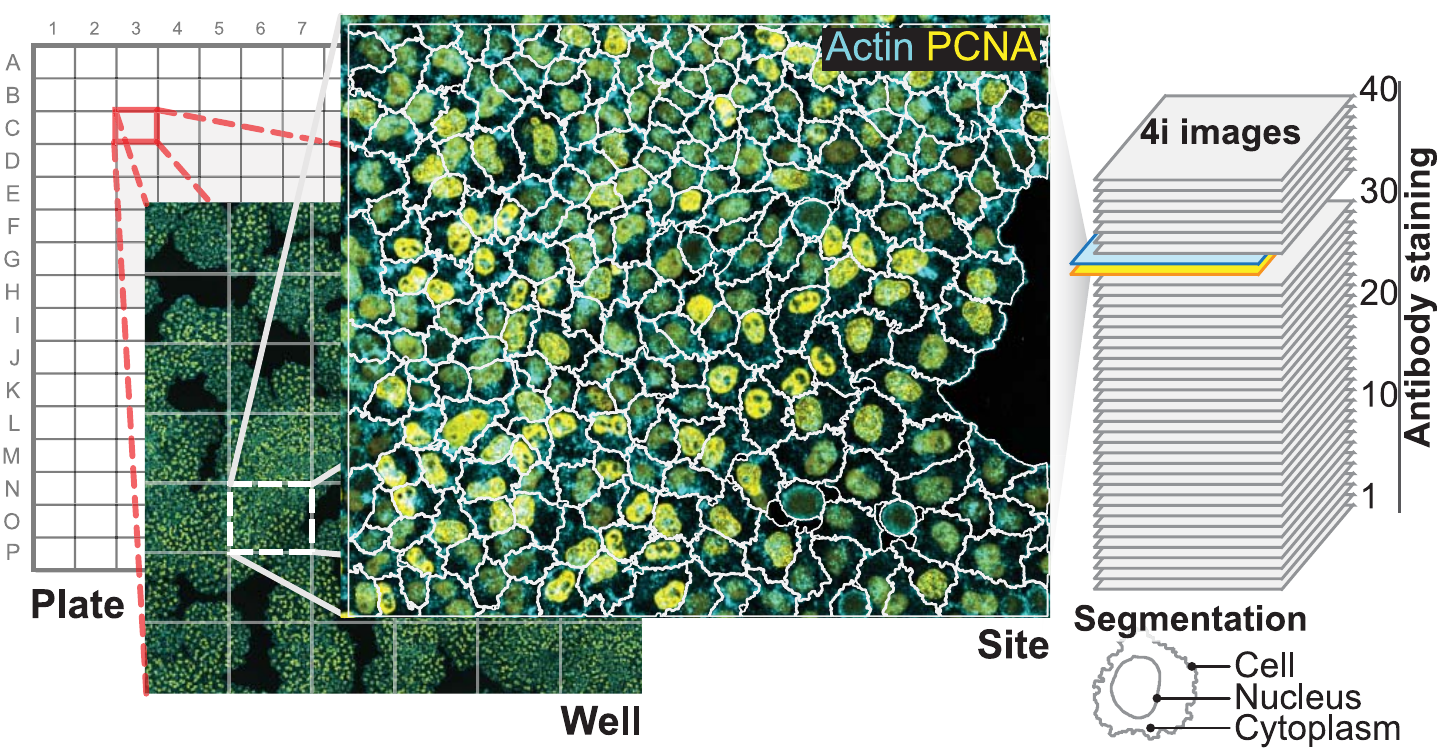
\includegraphics[width=100mm]{./Sections/Images/plate-well.png}
  \caption{\Acrlong{4i} process. Image source \cite{Guteaar7042}.}
  \label{fig:4i}
\end{figure}

Some technical details about \gls{4i}:
\begin{itemize}
  \item The images where obtained using a 40x objective and a \gls{scmos} camera, where the surface of each pixel is 165 nm by 165 nm.
  \item Each potho captures around 20,000 single cells.
  \item In \cite{Guteaar7042} (Fig 2), it is mentioned that use of 384-well plates, where wells were imaged at 40× magnification in a 7 × 6 tiled fashion for 21 4i cycles.
  \item The used cultured cells (tissue) where HeLa. HeLa is an immortal cell line used in scientific research.
\end{itemize}

The information for each single cell is not stored as a separated image as one may think, instead the information is first divided by Wells. Then, the information of the cells in a given well is stored in 7 files \fxnote{this is may not be included in the final work}:
\begin{itemize}
  \item \texttt{metadata.csv}: contains information of each cell in the well
  \item \texttt{channels.csv}: contains information of each protein (channel) photographed
  \item \texttt{labels.npy}: 1 dim array containing the cell label of each pixel
  \item \texttt{mpp.npy}: 2 dim array, where size of first dim is the same as number of measured pixels and size of second dim is the same as the number of channels. This file contains the observed measured values (intensities) of each pixel and for each protein. The values in \texttt{mpp.npy} vary from 0 to 65535 i.e. $2^{16}$ i.e. 2 bytes or 16 bits.
  \item \texttt{x.npy} and \texttt{y.npy}: 1 dim array containing the x/y coordinates of the measured pixels (pixels where a signal was detected by the \gls{scmos} camera. Accordingly with \cite{Guteaar7042}, the size of a single cell image (for each channel) is 2560x2160. Therefore, the values in \texttt{x.npy} vary between 1 and 2560 and form 1 to 2160 for \texttt{x.npy}
  \item \texttt{mapobject\_ids.npy}: 1 dim array where its size is the same as the number of rows in the \texttt{metadata.csv} file. Therefore, \texttt{mapobject\_ids.npy} maps the information given in the metadata file with each pixel in the well.
\end{itemize}

\textbf{QUESTION TO HANNAH:} In the paper it is mentioned that for each channel (protein), the tissue is stained with with 2 fluorescent antibodies (in that case TUBA1A and CTNNB1, NOT at the same time, TUBa1A-elution-CTNNB1), why? to create a background as reference for the protein that is being photographed?
Answer: To increase the measured signal, \ie to make the protein Shine more.

\section{Data Pre-processing}
\label{sec:Data_Preprocessing}

Since we are using a \gls{cnn} to predict the \gls{tr}, therefore we need the data as multichannel images. However, as we already explained in \ref{sec:Motivation_and_Background:Dataset}, the information is providad in a pixel by pixel format. Using the library \texttt{mpp\_data.py} written by Dr. Hannah Spitzer \fxnote{See how to refer properly to this library}, the raw data is transformed to multichannel images (one channel per protein measured). During this process, the bordered cells and cells in division process (Mitosis state) are excluded. The provided data set also contain the target variable, \ie the \gls{tr} (amount of \gls{mrna} molecules produced by the cell nucleus in the last 30 minutes). However, this information is coded also as a protein channel (00\_EU). Therefore, after converting the data set into multichannel images, the channel corresponding to the protein 00\_EU is extracted and converted into a number \fxnote{It is necessary to improve the description of how this 00\_EU channel is turned into a number. So far it is done by averaging all the entrances of the channel, however it still need to be decided if this will be done like this.}.
